\section{High Throughput Screening Results}

We next examined the remaining 67 elements identified in Figure \ref{Chap:Mg_H:fig4} (all elements with colors in the periodic table) with high-throughput DFT computations. Three successive rounds of calculations, each aimed at addressing one of the three criteria listed in Section 2.1, were conducted to narrow down the broader pool of elements highlighted in Figure \ref{Chap:Mg_H:fig4}. In the first round, we examined Fe segregation energies to determine which of the remaining elements in Figure \ref{Chap:Mg_H:fig4} prefers to segregate to bulk Fe rather than bulk Mg. This is the basis of the first criteria. In the second round, we determined which of those elements that passed the first round have favorable binding to Fe (100) and Fe (110) relative to bulk Fe. This is the basis of the second criterion. In the third and final round, we investigated which elements can either significantly weaken or strengthen H adsorption on Fe (110) and Fe (100).


For the first round, we calculated the second-phase particle segregation energy, $E_{particle seg}$,  of all alloying elements X (except As, which was previously addressed) denoted with colors in Figure \ref{Chap:Mg_H:fig4} using Equation \ref{Chap:Mg_H:eq:particle_seg}. As shown in Figure \ref{Chap:Mg_H:fig5}, elements with negative $E_{particle seg}$ are narrowed to 24: Be, B (Figure \ref{Chap:Mg_H:fig:5a}), Al, Si, P (Figure \ref{Chap:Mg_H:fig:5b}), Ti, V, Cr, Mn, Co, Ni, Ga, Ge, As (Figure \ref{Chap:Mg_H:fig5} (c)), Zr, Nb, Mo, Tc, Ru (Figure \ref{Chap:Mg_H:fig5} (d)), Hf, Ta, W, Re and Os (Figure \ref{Chap:Mg_H:fig5} (e)). No elements in the $7^{th}$ row or lanthanide series passed the first screening round (Figure \ref{Chap:Mg_H:fig5} (f)).


In the second round, we determined which of the 24 elements that passed the first screening round bind to Fe (100) and Fe (110) rather than to bulk Fe. The implication here is that potential slowing or even disruption of the HER can only occur if X preferentially binds to surfaces of Fe second-phase particles in an Mg alloy. We performed \ac{VASP} calculations with the remaining 24 elements adsorbed on Fe (100) and (110) using the models in Figure \ref{Chap:Mg_H:fig2} (c) and \ref{Chap:Mg_H:fig2} (d), where there is one atom of alloying element X in the top surface layer or the bulk layer of a (2x2) periodic unit cell. We calculated the surface segregation energy, $E_{surf seg}$, of all 24 elements using Equation \ref{Chap:Mg_H:eq:surf_seg}. According to Figure \ref{Chap:Mg_H:fig6}, only 13 elements from the pool of 24 from the second round were predicted to have favorable binding to Fe (100) ($E_{surf seg}$ < 0): Be, B, Al, Si, P (Figure \ref{Chap:Mg_H:fig6} (a)), Ti, Mn, Ni, Ga, Ge, As (Figure \ref{Chap:Mg_H:fig6} (b)), Zr (Figure \ref{Chap:Mg_H:fig6} (c)), and Hf (Figure \ref{Chap:Mg_H:fig6} (d)). Figure \ref{Chap:Mg_H:fig6} (c) suggests that Nb has no preference for either Fe (100) or bulk Fe. We passed Nb on, nevertheless, to the third screening round. Similarly, Figure 7 shows the same 13 candidates for Fe (110).  Hence, Be, B, Al, Si, P, Ti, Ni, Ga, Ge, As, Zr, Nb, and Hf are passed to the third and final screening round.


\begin{table}[ht]
\caption[Summary of H adsorption energies (eV/atom) defined at Equation \ref{Chap:Mg_H:eq:H_ads} at selected sites on (2$\times$2) Fe (100) and Fe (110) surface slabs without/with one substitutional atom from one of the 13 alloying elements that pass the second screening round.]{Summary of H adsorption energies (eV/atom) defined at Equation \ref{Chap:Mg_H:eq:H_ads} at selected sites on (2$\times$2) Fe (100) and Fe (110) surface slabs without/with one substitutional atom from one of the 13 alloying elements that pass the second screening round. H adsorption site is indicated at the top of each column and plotted in Figure 3(a) and 3(b). The ``stability'' at the top of the $5^{th}$ column means that H stays at the hollow site I on Fe (110) with substitutional alloying atoms as Figure 3(b) after the H and surface atoms are fully relaxed by \ac{VASP} optimization. Otherwise, the H adsorption energies at such hollow site I are calculated by only allowing the H and surface atoms to relax in the direction normal to the surface.}
\label{Chap:Mg_H:tab:H_ads}
\centering
\begin{tabular}{cccccc}
\\
\hline
\hline
        & \begin{tabular}[c]{@{}c@{}}(100) \\ top site\end{tabular} & \begin{tabular}[c]{@{}c@{}}(100) \\ hollow site\end{tabular} & \begin{tabular}[c]{@{}c@{}}(110)\\  top site\end{tabular} & \begin{tabular}[c]{@{}c@{}}(110) hollow \\ site I stability\end{tabular} & \begin{tabular}[c]{@{}c@{}}(110) hollow \\ site I\end{tabular} \\ \hline
Pure Fe & 0.2                                                       & -0.38                                                        & 0.02                                                      & Yes                                                                      & -0.71                                                          \\
Be      & 0.34                                                      & -0.4                                                         & -0.14                                                     & Yes                                                                      & -0.65                                                          \\
B       & -0.01                                                     & -0.4                                                         & -0.29                                                     & No                                                                       & -0.3                                                           \\
Al      & 0.03                                                      & -0.31                                                        & 0.72                                                      & No                                                                       & -0.29                                                          \\
Si      & -0.18                                                     & -0.26                                                        & 0.68                                                      & No                                                                       & -0.11                                                          \\
P       & 0.13                                                      & -0.31                                                        & 0.83                                                      & No                                                                       & 0.3                                                            \\
Ti      & 0.26                                                      & -0.43                                                        & 0.7                                                       & No                                                                       & -0.37                                                          \\
Ni      & 0.1                                                       & -0.46                                                        & -0.08                                                     & Yes                                                                      & -0.53                                                          \\
Ga      & 0.2                                                       & -0.28                                                        & 0.82                                                      & No                                                                       & 0.02                                                           \\
Ge      & 0.23                                                      & -0.24                                                        & 0.82                                                      & No                                                                       & 0.28                                                           \\
As      & 0.67                                                      & -0.22                                                        & 0.81                                                      & No                                                                       & 0.61                                                           \\
Zr      & 0.28                                                      & -0.44                                                        & 0.62                                                      & No                                                                       & 0.37                                                           \\
Nb      & 0.01                                                      & -0.41                                                        & 0.35                                                      & No                                                                       & -0.22                                                          \\
Hf      & 0.15                                                      & -0.42                                                        & 0.53                                                      & No                                                                       & 0.14                                                           \\ \hline\hline
\end{tabular}
\end{table}


In the third screening round, we investigated the H adsorption energies on both Fe (100) and Fe (110) with each of the 13 elements that passed the second screening round. Results are shown in Figure 8 and Table \ref{Chap:Mg_H:tab:H_ads}. We used Equation \ref{Chap:Mg_H:eq:H_ads} to calculate the H adsorption energies $E_{ad}^H$ on the two Fe surfaces with 1 alloying element X substituting a surface Fe atom as shown in Figs. \ref{Chap:Mg_H:fig3} (a) and \ref{Chap:Mg_H:fig3} (b). Based upon our results for As, we limited the number of models for each Fe surface to two: H at the hollow site and at the top site of an alloying element X adsorbed on Fe (100) (Figure \ref{Chap:Mg_H:fig3} (a)), H at the hollow site I and at the top site of an alloying element X adsorbed on Fe (110) (Figure \ref{Chap:Mg_H:fig3} (b)). In the instance that an element X caused H to move from the hollow site I to the hollow site II on Fe (110), the same as the case for As, we only relaxed the H and the surface atoms along the direction normal to the surface to calculate $E_{ad}^H$. This decision was made after we fully relaxed all atoms on Fe (110) and determined which X causes H to move from its initial position. Whether to apply this restriction is summarized in Table \ref{Chap:Mg_H:tab:H_ads}, which uses the column of ``(110) hollow site I stability'' to indicate whether the H atom stays in the hollow site I (``Yes'' in that column) or moves to another site (``No'' in that column) after full relaxation.


Figure \ref{Chap:Mg_H:fig8} shows H adsorption energies at hollow sites (the solid horizontal lines in both Figure \ref{Chap:Mg_H:fig8} (a) and \ref{Chap:Mg_H:fig8} (b)) and top sites (the dashed horizontal lines in both Figure \ref{Chap:Mg_H:fig8} (a) and \ref{Chap:Mg_H:fig8} (b)) on both pure Fe (100) and (110) surfaces, indicating that H prefers the hollow sites rather than the top sites. The same trend can be found for Fe surfaces with one of the 13 alloying element X as shown by the curved lines with open (for H at top sites) /solid (for H at hollow sites) circles in both Figure \ref{Chap:Mg_H:fig8} (a) and \ref{Chap:Mg_H:fig8} (b). The numerical values of the corresponding $E_{ad}^H$ for each case are listed in Table \ref{Chap:Mg_H:tab:H_ads}. Thus, the hydrogen adsorption energy at the hollow site was used as a numerical criterion to determine whether an alloying element can increase or reduce the hydrogen adsorption strength on Fe surfaces. For the Fe (100) surface, 6 of the 13 remaining alloying elements (As, Ge, Ga, P, Si, Al) resulted in a significant reduction of hydrogen adsorption strength on the hollow site, all of which have $E_{ad}^H$ values more positive than $E_{ad}^H$ for H at the hollow site on pure Fe (100) as shown in Figure \ref{Chap:Mg_H:fig8} (a). The other 7 alloying elements (Be, B, Ti, Ni, Zr, Nb, and Hf) resulted in almost no changes or even slightly increased the hydrogen adsorption strength.


On Fe (110), the addition of an element X may cause H to move, as was observed for As. This had the net result of moving the H from hollow site I to hollow site II in Figure \ref{Chap:Mg_H:fig3} (b). Interestingly, Be and Ni were the notable exceptions in the pool of the 13 alloying elements X investigated in the third screening round since H remained at hollow site I in the presence of either element as indicated by the ``Yes'' in the column of ``(110) hollow site I stability'' of Table \ref{Chap:Mg_H:tab:H_ads}. Comparison of the pure Fe (110) H adsorption energy of -0.71 eV at hollow site I with H adsorption energies at the same site on Fe (110) with one of the 13 X implies that each of these elements weakens H adsorption strength on an Fe surface. Moreover, this comparison leads to the following rank ordering of the 13 elements starting with As, which causes the greatest weakening of H adsorption strength, and ending with Be that weakens H adsorption strength the least: $\text{As} > \text{Zr} > \text{Ge} \approx \text{P} > \text{Hf} > \text{Ga} > \text{Si} > \text{Nb} > \text{Al} > \text{B} > \text{Ti} > \text{Ni} > \text{Be}$.


Comparison of the H adsorption energies between the (100) hollow site and (110) hollow site identifies six elements that significantly weaken or destabilize H adsorption on both Fe (100) and Fe (110) are: Al, Si, P, Ga, Ge, As. The inference here is that they will reduce \ac{HER} rates on both Fe surfaces by slowing the Volmer reaction in Equation \ref{Chap:Mg_H:eq:Tafel}. Transition metal elements (Ti, Ni, Zr, Nb, and Hf) and B can have opposite effects on hydrogen adsorption strengths on Fe (100) and Fe (110) surfaces, and hence changes to the \ac{HER} rate are likely to be quite small. Specifically, changes in hydrogen adsorption energies on Fe (100) with these transition metal elements are relatively minor, which are confirmed by further studies of Fe (100) with higher surface concentrations of substitutional alloying atoms in Sec. 4. Hence, these surfaces can still behave as active cathode sites with a fast \ac{HER} rate, resulting in their elimination from the candidate list of potential corrosion inhibitors. Beryllium has the most favorable H adsorption energies at both the Fe (110) hollow site I (-0.65 eV/atom) and the Fe (100) hollow site (-0.40 eV/atom) relative to corresponding H adsorption energies on the pure Fe surfaces (-0.71 eV atom for the Fe (110) hollow site I and -0.38 eV/atom at the Fe (100) hollow site), resulting in its elimination from the list.


Since all of the H adsorption energies on hollow sites of the alloyed Fe (100) (Figure \ref{Chap:Mg_H:fig3} (a)) are obtained based on VASP relaxations with no ancillary restrictions, we expect that these adsorption energies can be used to rank the order the final six elements (Al, Si, P, Ga, Ge, As) based upon reduction and/or destabilization of H adsorption to the Fe surfaces. According to the results in Table \ref{Chap:Mg_H:tab:H_ads}, these H adsorption energies suggest the following rank ordering by reduction of H adsorption strengths, and consequently, HER rates as: $\text{As} > \text{Ge} > \text{Si} > \text{Ga} > \text{P} \approx \text{Al}$. These p-block elements, which are highlighted in green in Figure \ref{Chap:Mg_H:fig4}, are the final group of corrosion-inhibiting elements that resulted from the application of the three criteria discussed above in our high-throughput computations. Note that the high-throughput computations call out As and Ge as potentially the best corrosion inhibiting elements using the idealized models in Figure \ref{Chap:Mg_H:fig2} and \ref{Chap:Mg_H:fig3}.


This result is in qualitative accord with experiments \cite{liu2016controlling,birbilis2014evidence}. A recent experimental study shows that microalloying additions of Ge, Sb, Pb, Sn, and Bi (group 14 and 15 elements) can reduce the cathodic kinetics upon Mg, and Mg-Ge alloys were demonstrated to have the highest corrosion resistance among them \cite{liu2018simultaneously}. Another experimental study on corrosion behavior of biodegradable Mg–X (X = Sn, Ga, In) alloys shows a low amount ($<$ 1 wt$\%$) of Ga is the most effective among these three elements to improve the corrosion resistance of Mg alloys \cite{kubasek2013structure}. We didn't consider the effects of In, Sn, Sb, Pb or Bi in our studies because our \ac{VASP} calculations suggest that these four elements prefer to stay in Mg matrix instead of Fe particles (Figure \ref{Chap:Mg_H:fig4} and \ref{Chap:Mg_H:fig5}). In reality, even Sn, Sb, Pb and Bi may prefer to stay on the surfaces of Fe-rich particles relative to the Mg matrix due to surface segregation, and hence it possible that they reduce the cathodic kinetics to some extent.

\newpage
\begingroup
\begin{figure}[!ht]
  \centering
  \subfigure[]{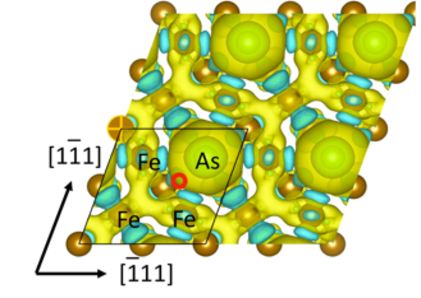
\includegraphics[width=0.45\linewidth]{Chap3/plots/Fig9a.pdf}}\label{Chap:Mg_H:fig:9a}
  \subfigure[]{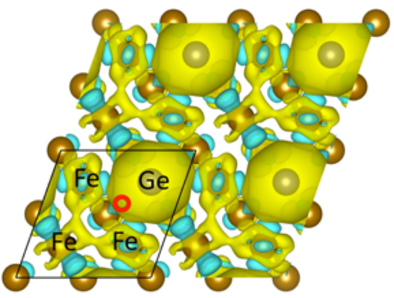
\includegraphics[width=0.45\linewidth]{Chap3/plots/Fig9b.pdf}}\label{Chap:Mg_H:fig:9b}
  \\
  \subfigure[]{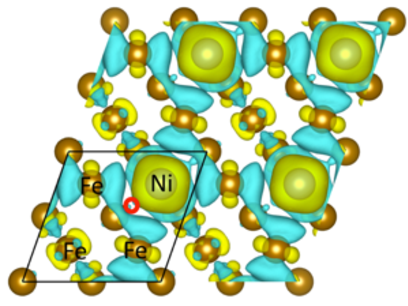
\includegraphics[width=0.45\linewidth]{Chap3/plots/Fig9c.pdf}}\label{Chap:Mg_H:fig:9c}
  \subfigure[]{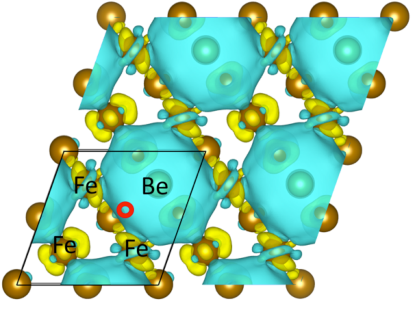
\includegraphics[width=0.45\linewidth]{Chap3/plots/Fig9d.pdf}}\label{Chap:Mg_H:fig:9d}
\caption[Top-down views of isosurfaces of electron density difference for (2x2) Fe (110) with one substitutional alloying atom in top surface layer]{Top-down views of isosurfaces of electron density difference ($\Delta \rho$ defined in Equation \ref{Chap:Mg_H:eq:chargediff}) for (2x2) Fe (110) with one substitutional alloying atom in top surface layer. Surface Fe and alloy element X (X as As, Ge. Ni and Be in (a), (b), (c) and (d), respectively) are denoted. The open red circle is located at a hollow site I (Figure \ref{Chap:Mg_H:fig3} (b)) for hydrogen adsorption. The black box indicates the periodicity of a (2x2) Fe (110). The yellowish isosurface is $1.5x10^{-3}\frac{e}{bohr^3}$ corresponding to positive $\Delta \rho$ or electron accumulation after the substitutional alloying. The blue isosurface is $-1.5x10^{-3}\frac{e}{bohr^3}$ corresponding to negative $\Delta \rho$ or electron depletion after the substitutional alloying.}
  \label{Chap:Mg_H:fig9}
\end{figure}
\endgroup





